\documentclass{sig-alternate-sigmod09}

\usepackage[bookmarks=true,pdfborder= 0 0 0]{hyperref}

\usepackage{tikz}
\usetikzlibrary{calc,trees,positioning,arrows,chains,shapes.geometric,%
  decorations.pathreplacing,decorations.pathmorphing,shapes,%
  matrix,shapes.symbols,plotmarks,decorations.markings,shadows}

\DeclareMathOperator{\atantwo}{atan2}

\hypersetup{
pdfauthor={Patrick Brosi},
pdfkeywords=,
pdftitle={Metro Maps on Octilinear Grid Graphs},
pdfsubject={},
pdfcreator={},
pdfproducer={}
}

\newcommand\todo[1]{\textcolor{blue}{[TODO: #1]}}
\newcommand\TODO[1]{\textcolor{blue}{\small [TODO: #1]}}

% Input Graph

\def\iG{G}  % Input graph
\def\iV{V}  % Input nodes
\def\iv{v}  % Input node
\def\iE{E}  % Input edges
\def\ie{e}  % Input edge

% Drawing

\newcommand\drawing[1]{\mathcal{D}_{#1}}  % Drawing of graph
\newcommand\initdrawing[1]{\drawing{#1}^*}  % Drawing of graph

\def\drawingcurvesym{c}  % edge curve part of drawing
\def\drawingpossym{p}    % node position part of drawing

\newcommand\drawingcurve[1]{\drawingcurvesym(#1)}  % Drawing curve of argument edge
\newcommand\drawingpos[1]{\drawingpossym(#1)}  % Drawing pos urve of argument node

% Grid

\def\gScale{C}
\def\gmind{\hat d}


% Octilinear grid graph

\def\gG{\Gamma}  % Grid graph
\def\gV{\Psi}  % Grid graph nodes
\def\gv{\psi}  % Grid graph node
\def\gE{\Omega}  % v edges
\def\ge{\omega}  % Grid graph edge

\newcommand\ggv[2]{\gv_{#1, #2}}  % Grid node at #1, #2
\newcommand\gpv[3]{\gv_{#1, #2}^{#3}}  % Port #3 node at #1, #2
\newcommand\gse[3]{\ge_{#1, #2}^{#3}}  % Sink edge #3 node at #1, #2
\newcommand\gbe[4]{\ge_{#1, #2}^{#3, #4}}  % Bend edge for angle #4 at port #3 at node at #1, #2

\def\gPath{p}    % path on grid graph
\def\gPathOcti{p'}    % path on octilinear grid graph

\newcommand\gPturn[1]{c_{#1}}  % Turn penalty
\newcommand\gPturnEdge[1]{c'_{#1}}  % Turn penalty
\def\gHopcost{c_h}    % Hop cost in grid graph
\def\gHopcostOcti{c'_h}    % Hop cost in grid graph
\def\gSinkcost{c_s}    % Hop cost in grid graph
\newcommand\gPcost[1]{c(#1)}  % Path cost
\newcommand\gPcostOcti[1]{c'(#1)}  % Octilinear path cost

% ILP

\newcommand\gvused[2]{x_{#1#2}}	% bin. decision variable whether grid node #1 is assigned to input node #2
\newcommand\geused[2]{x_{#1#2}}	% bin. decision variable whether grid edge #1 is used be input edge #2

\newcommand\dir[2]{\delta_{#1#2}}	% variable telling the direction of edge #2 at node #1
\newcommand\dirdiff[2]{\Delta_{#1#2}}	% variable telling the direction difference of edge #1 and edge #2

\newcommand\bend[3]{\Delta_{#1#2}^{#3}}	% variable telling the direction difference of edge #1 and edge #2

\def\ldeg{\text{ldeg}}

\begin{document}
\title{Metro Maps on Octilinear Grid Graphs}
\subtitle{- sketch -}

\numberofauthors{1}
%\author{Patrick Brosi\\\affaddr{University of Freiburg}\\\affaddr{Chair of Algorithms and Data Structures}}

\maketitle

\section{Abstract}

We investigate a novel approach to the problem of drawing octilinear Metro Maps.
We state the problem as a batch of shortest-path calculations on a specially crafted octilinear grid graph, where edge bends are added to the total cost of the path by means of explicit turn edges.
Our approach can be optimized exactly via an Integer Linear Program (ILP) or approximately by iteratively calculating shortest-paths between node candidates in the octilinear grid graph.
Most importantly, it allows us to revisit earlier work [Stott] which used local search techniques to update the node positions until a (local) optimum was found, but where octilinearity was not guaranteed.
By recalculating the shortest-path between an updated node and its neighbors on our octilinear grid graph, we can guarantee octilinearity.
Using this approach, we can calculate metro maps which are very close to optimal in a fraction of a second even for large networks.
As far as we are aware, our technique is the first non-global approach which guarantees octilinear results, albeit at the cost of not always finding a solution.
%Our maps are rendered using previous work and are publicly accessible.

\section{Introduction}

\TODO{Write intro}

\subsection{Problem definition}

Given an undirected planar input graph $\iG = (\iV, \iE)$, where $\iV$ are stations (or other location of interests in a public transit network) and $\iE$ are connections between those stations.
We say $\drawing{\iG} = (\drawingpossym, \drawingcurvesym)$ is a drawing of $\iG$, where $\drawingpos{\iv}$ assigns a position to every node $\iv \in \iV$ and $\drawingcurve{\ie} = (q_0, q_1, ..., q_n)$ assigns a piecewise linear curve to every edge $\ie \in \iE$.
The initial input drawing $\initdrawing{\iG}$ assigns each node a geographical real-world position, and each edge an (optional) real-world trajectory.
\TODO{mention line labels and use same definition as in LOOM paper}
Our goal is to find a schematic drawing $\mathcal{D}'_G$ that resembles a classic Metro Map.
This is usually formalized as a set of hard and soft constraints \cite{nb, ...}.
The hard constraints may be summarized as:
\begin{enumerate}
\setlength\itemsep{.1em}
\item \emph{Octilinearity}. Each edge curve $\drawingcurve{\ie}$ may only consist of segments whose orientation is a multiple of $45^{\circ}$.
\item \emph{Topology preservation}. The input embedding should be respected. In particular, no crossings between edges should be introduced and non-incident edges should never share common points.
\end{enumerate}
Additionally, the following soft constraints are usually employed:
\begin{enumerate}
\setlength\itemsep{.1em}
\item \emph{Edge monotony}. The number of edge bends should be minimized and large angles preferred.
\item \emph{Geographical accuracy}. The original node positions should be changed as little as possible.
\item \emph{Map density}. There should be a minimum distance $\gmind$ between the anchor points of curves to ensure readability.
\end{enumerate}

With respect to edge monotony and octilineary, previous work often defined the problem as finding an octilinear embedding of the input graph, where each edge is represented by a straight octilinear arc.
We use a slightly different approach and state the problem as finding the optimal posititions $p(v) \in \mathbb{N}^2$ on a grid for each station node and curves $c(e) = (q_0, q_1, ..., q_n)$, $q_i \in \mathbb{N}^2$ connecting them. 
Most importantly, for two suceeding points $q_i = (x_i, y_i)$ and $q_{i+1} = (x_{i+1}, y_{i+1})$, we require that they have a distance of 1 with respect to the uniform norm $L^{\infty}$.
This means that the distance $|q_{i+1} - q_{i}|_{\infty}$ between them is defined as $\max \{|x_{i+1} - x_i|, |y_{i+1} - y_i|\}$.
For any point on the grid, the distance to all its 8 direct neighbors is thus 1.

To project this grid onto a map plane, we use a scale factor $\gScale$, which is essentially the height and length of a grid cell.
If $\gScale$ is set to $\gmind$, a minimum distance between any two grid points is guaranteed to be greater or equal to $\gmind$.

\subsection{Related Work}

Survey Noellenburg %http://i11www.iti.kit.edu/extra/publications/n-asamm-14.pdf
Survey Wolff %http://www1.pub.informatik.uni-wuerzburg.de/pub/wolff/pub/w-dsms-07.pdf
Hong et al., force-based approach
Stott's PhD
steiner trees! %https://www.researchgate.net/profile/Matthias_Mueller-Hannemann/publication/225160153_Approximation_of_Octilinear_Steiner_Trees_Constrained_by_Hard_and_Soft_Obstacles/links/0912f50cf248ec1193000000/Approximation-of-Octilinear-Steiner-Trees-Constrained-by-Hard-and-Soft-Obstacles.pdf

\section{Octilinear Grid Graph}

\begin{figure*}[t]
  \centering
	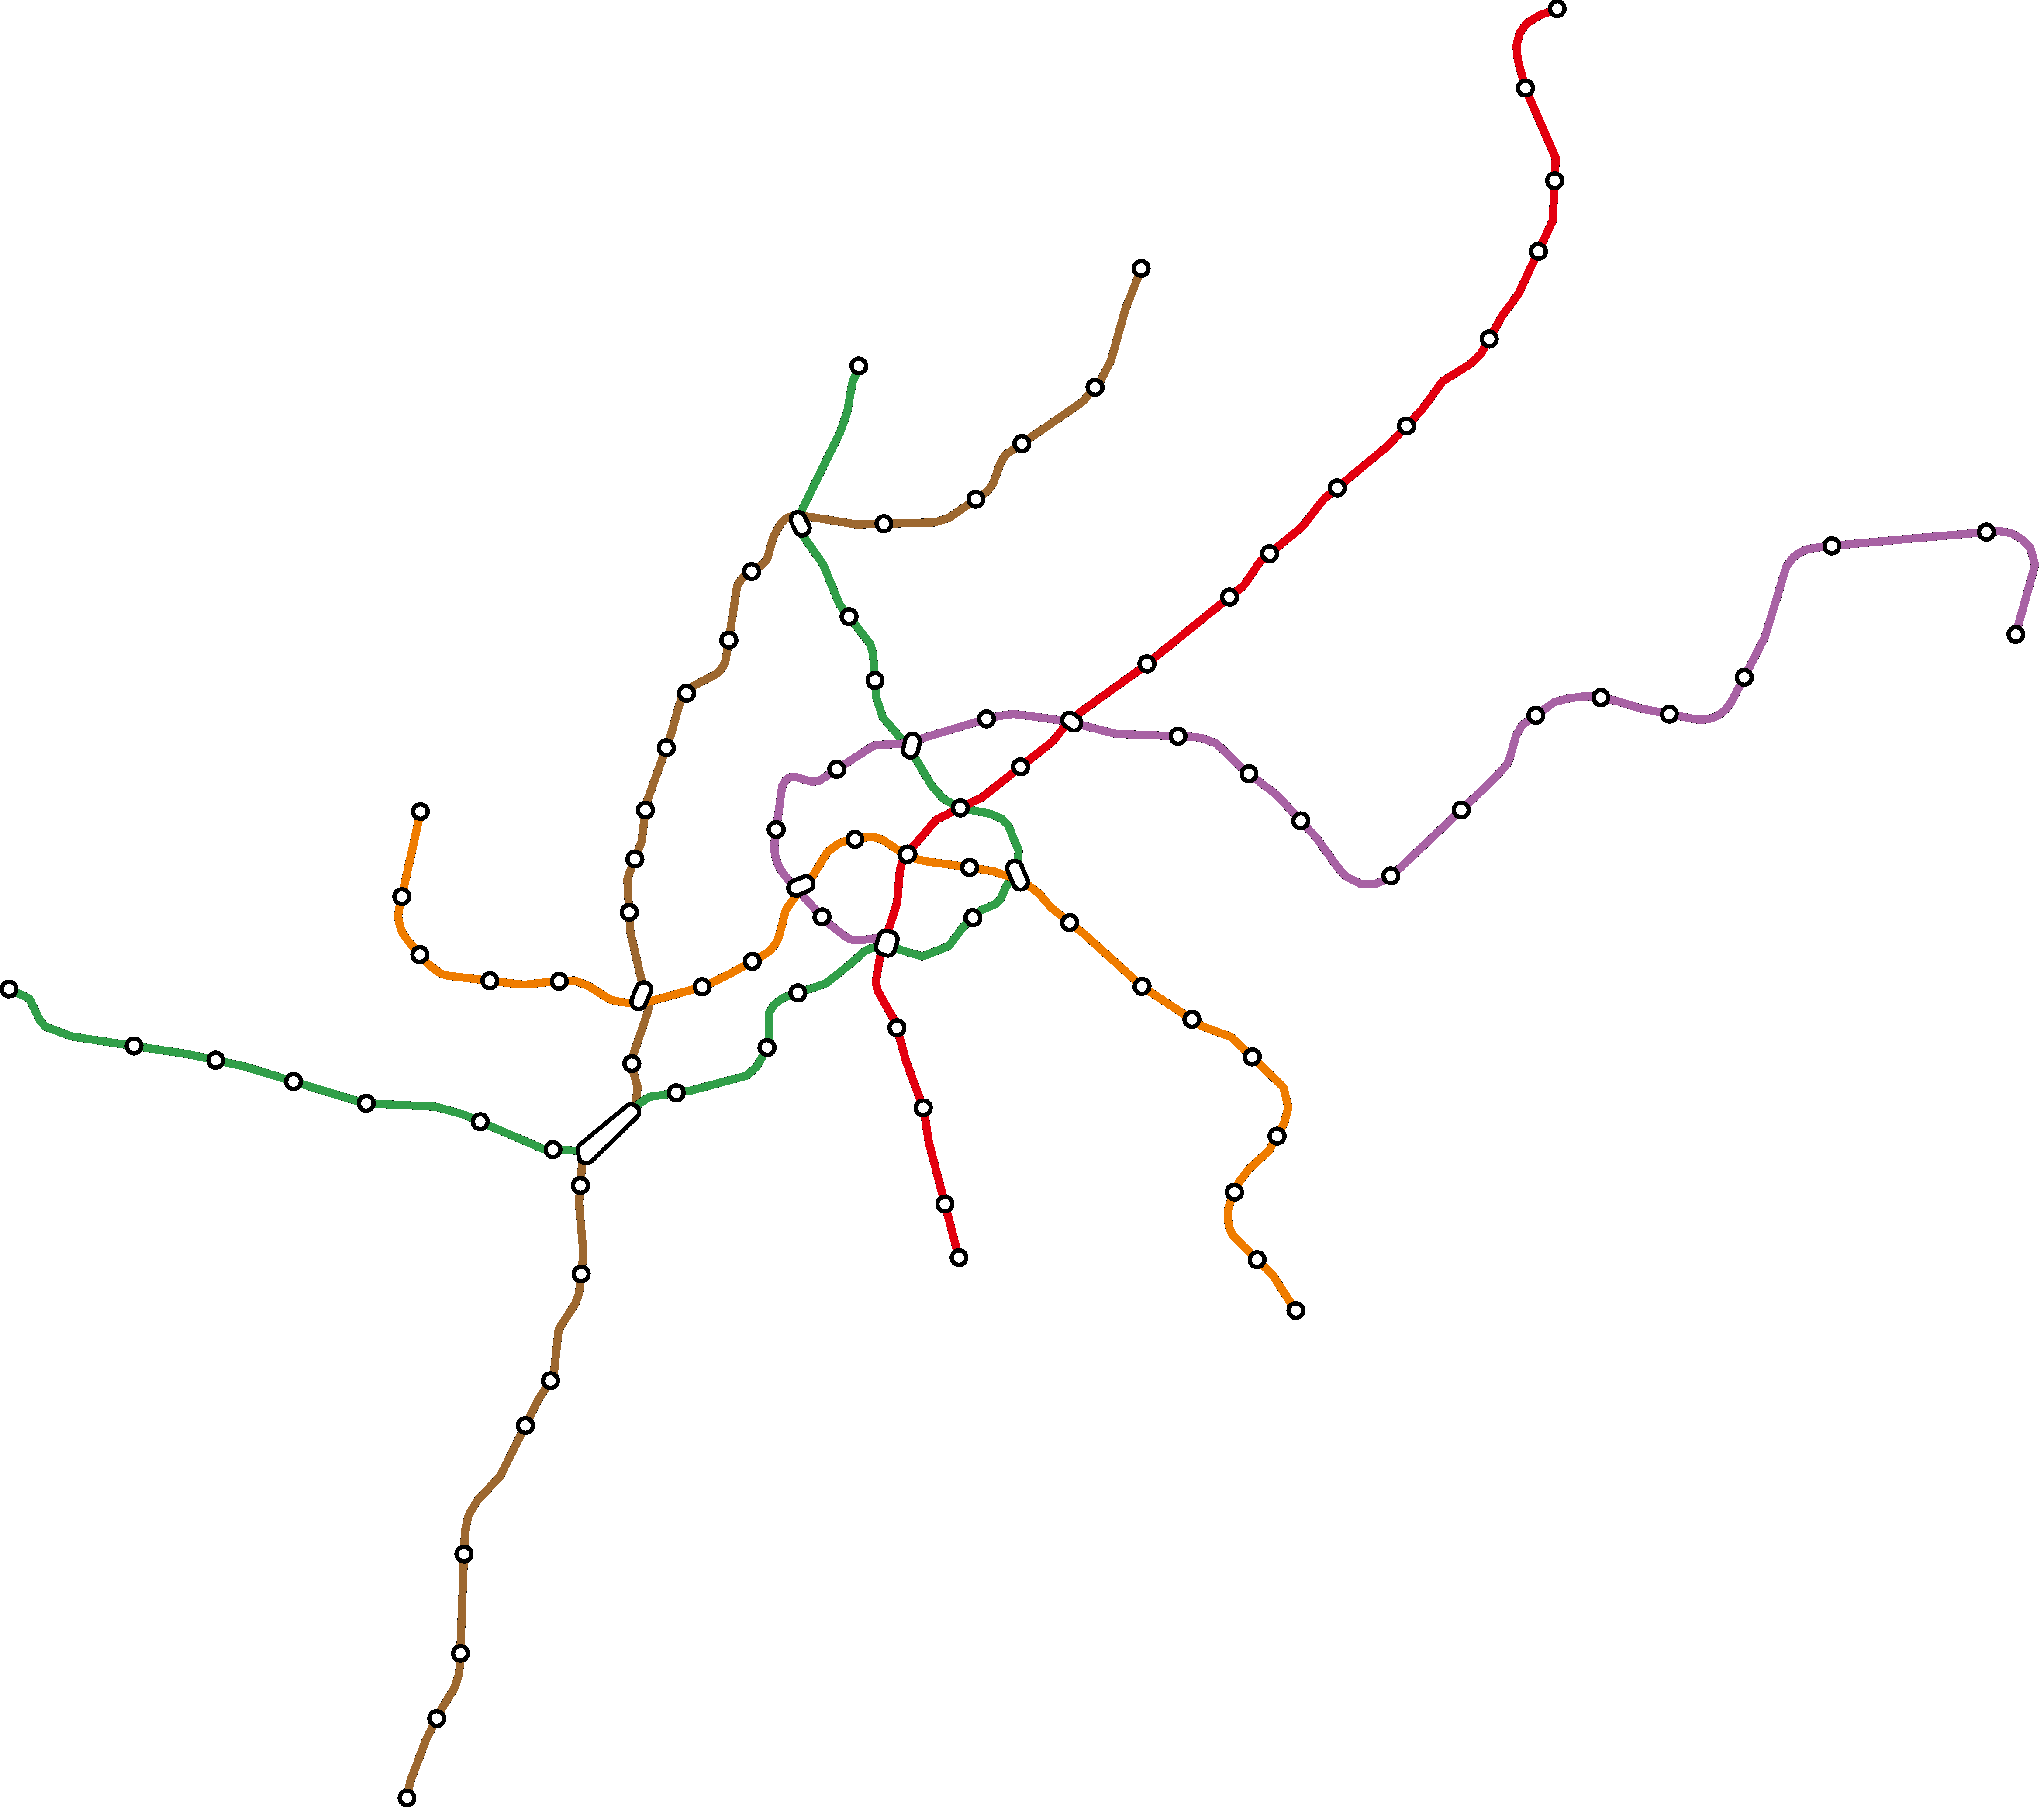
\includegraphics[width=0.474\textwidth]{figures/octi_input.pdf}
	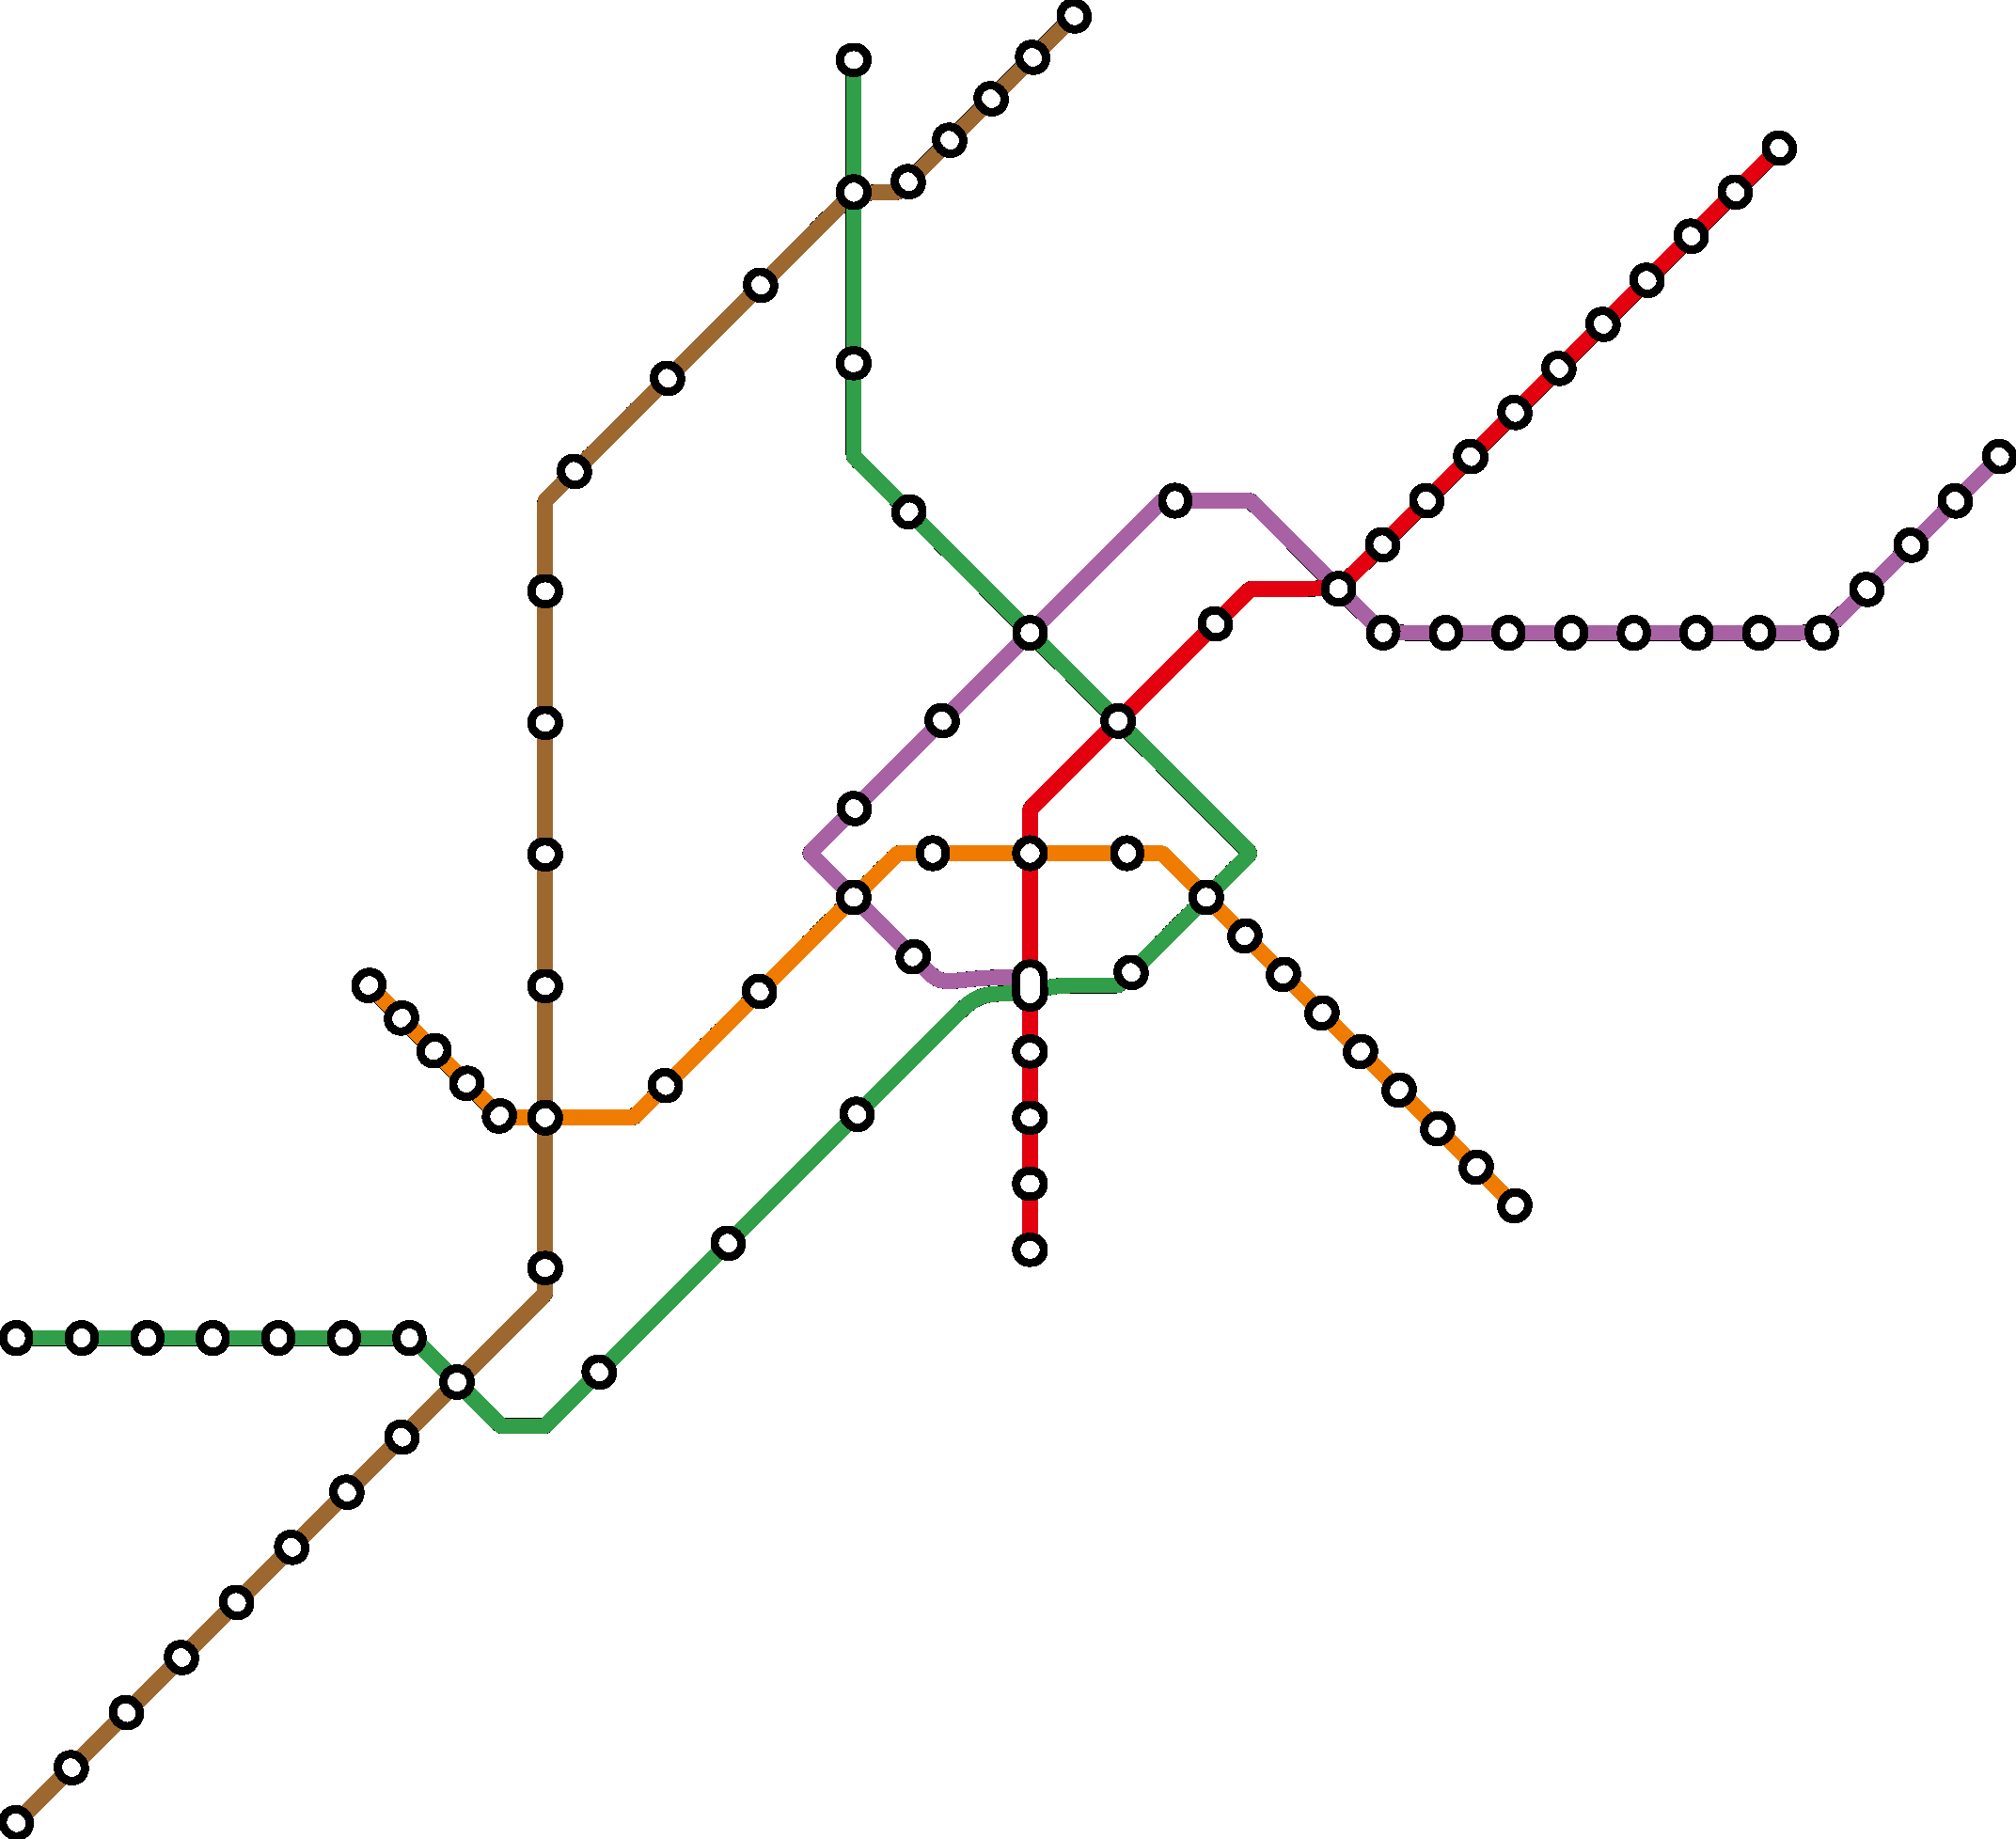
\includegraphics[width=0.474\textwidth]{figures/octi.pdf}
	\caption{The subway network of Vienna, rendered with our approach from raw timetable (GTFS) data (including stop positions).}
	\label{FIG:examplewien}
\end{figure*}

We use an auxiliary undirected graph $\gG = (\gV, \gE)$, where $\gV$ is the set of nodes and $\gE$ is the set of edges and in which every possible path $\gPath = (\gv_0, \gv_1, ..., \gv_n), \gv_i \in \gV$ with $\gv_0 \neq \gv_n$ and $|\gPath| > 1$ represents an octilinear curve with cost $\gPcost{\gPath} = (n - 1) \cdot \gHopcost$, where $\gHopcost$ is the ``hop'' cost of using a single edge.
The graph in Fig.~\ref{FIG:gridgraph},~left trivially satisfies this: we define a $X\times Y$ grid and add nodes $\ggv{x}{y}$ for every grid point.
Each node $\psi_{x,y}$ is connected with its 8 direct neighbors (except at the grid boundaries) $N^0(\ggv{x}{y}) ... N^7(\ggv{x}{y})$, where $N^0(\ggv{x}{y})$ is the ``north'' neighbor of $\ggv{x}{y}$, $N^1(\ggv{x}{y})$ the ``north-east'' neighbor etc..

\subsection{Penalizing Line Bends}

To later be able to optimize soft constraint (1), we additionally want the total cost for a path in $\Gamma$ to reflect the number and accuteness of bends.
The penalty for a turn should be weighted by its degree - either $135^{\circ}$, $90^{\circ}$ or $45^{\circ}$.
We call these penalties $\gPturn{135}$, $\gPturn{90}$ and $\gPturn{45}$.
A straight pass through a node should go unpunished, so $\gPturn{180} = 0$.
Since we aim for a ``smooth'' path through $\gG$ and want to favor obtuse angles, we require $\gPturn{180} \leq \gPturn{135} \leq \gPturn{90} \leq \gPturn{45}$.

We extend our cost function and now search for the path $\gPath = (\gv_0, \gv_1, ..., \gv_i, ..., \gv_n)$ which minimizes
\begin{align}
	\gPcost{\gPath} = (n - 1) \cdot \gHopcost + \sum_{i=1}^{n - 1} t(\gv_{i-1}, \gv_{i+1}),
\end{align}
where $t(\gv_{i-1}, \gv_{i+1})$ is the angular turn cost between edges $\{\gv_{i-1}, \gv_{i}\}$ and $\{\gv_{i}, \gv_{i=1}\}$, that is, either 0, $\gPturn{135}$, $\gPturn{90}$ or $\gPturn{45}$.

\begin{figure}
  \centering
	$\vcenter{\hbox{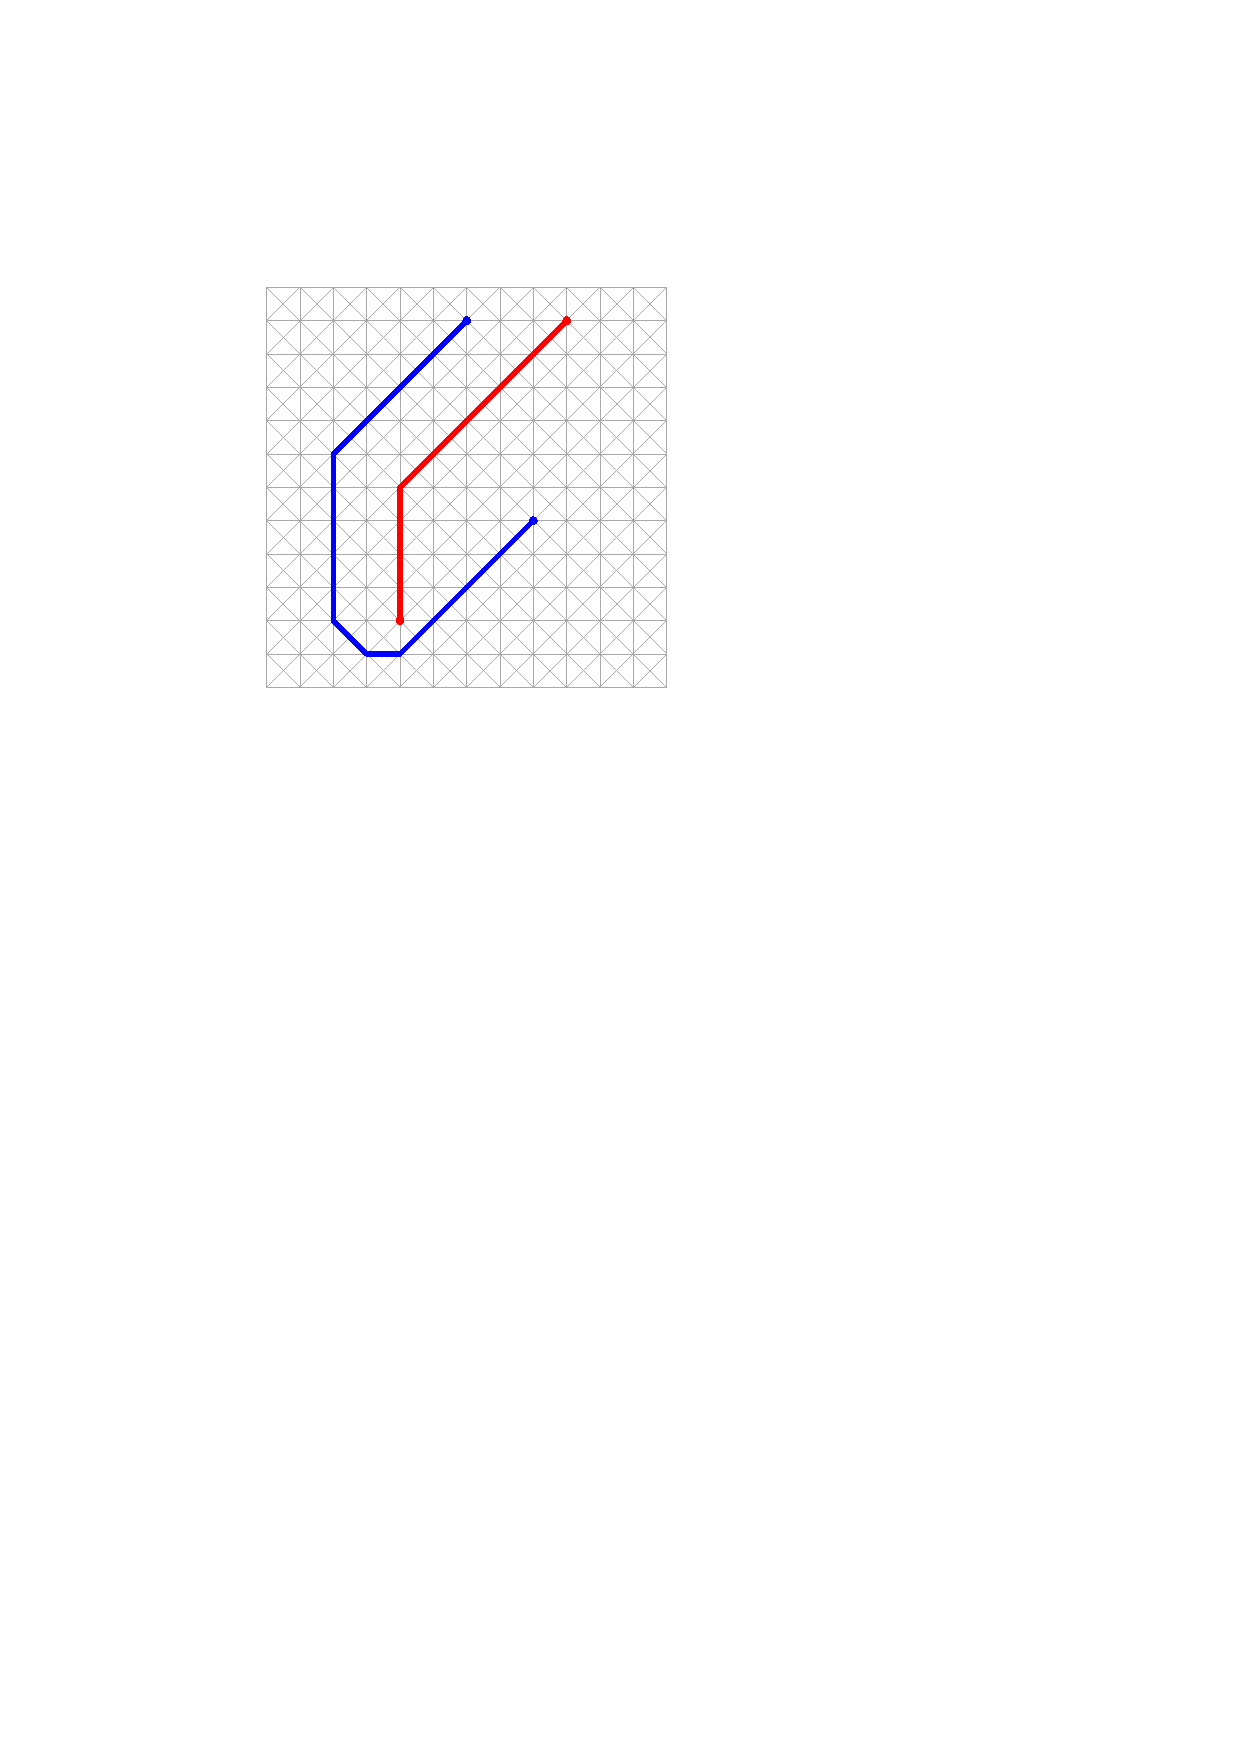
\includegraphics[width=0.474\textwidth]{figures/grid.pdf}}}$
	\caption{Left: A shortest path between $t$ and $u$ on a grid graph with uniform edge cost. Path bends are not minimized. Right: Two shortest path between $(t, u)$, and $(v, w)$ on our octilinear grid graph with uniform grid edge cost $1$ and additional path turn penalties $p_{135} = 1$, $p_{90} = 1.5$ and $p_{45} = 2$. Path $(t, u)$ acts as an obstacle for $(v, w)$.}
	\label{FIG:grids}
\end{figure}

We model this by adding 8 auxiliary port nodes $\gpv{x}{y}{0} ... \gpv{x}{y}{7}$ to every grid node (Fig.~\ref{FIG:gridgraph}).
Each port again corresponds to an outgoing angle in clockwise fashion and is connected to $\ggv{x}{y}$ via sink edges $\gse{x}{y}{0} ... \gse{x}{y}{7}$.
These sink edges allow us to leave from and arrive at an original node $\psi_{x, y}$.
For paths passing through the original grid node $\ggv{x}{y}$, we connect each port $\gpv{x}{y}{i}$ with its 7 - i suceeding (in clockwise fashion) sibling ports with turn edges $\omega_{x, y}^{i@45}$, $\omega_{x, y}^{i@90}$, and so forth.
For ease of notation, we allow a turn edge to be identified by both its port nodes, for example, $\omega_{x, y}^{0@45} = \omega_{x, y}^{1@45}$.

\begin{figure}[b]
  \centering
	$\vcenter{\hbox{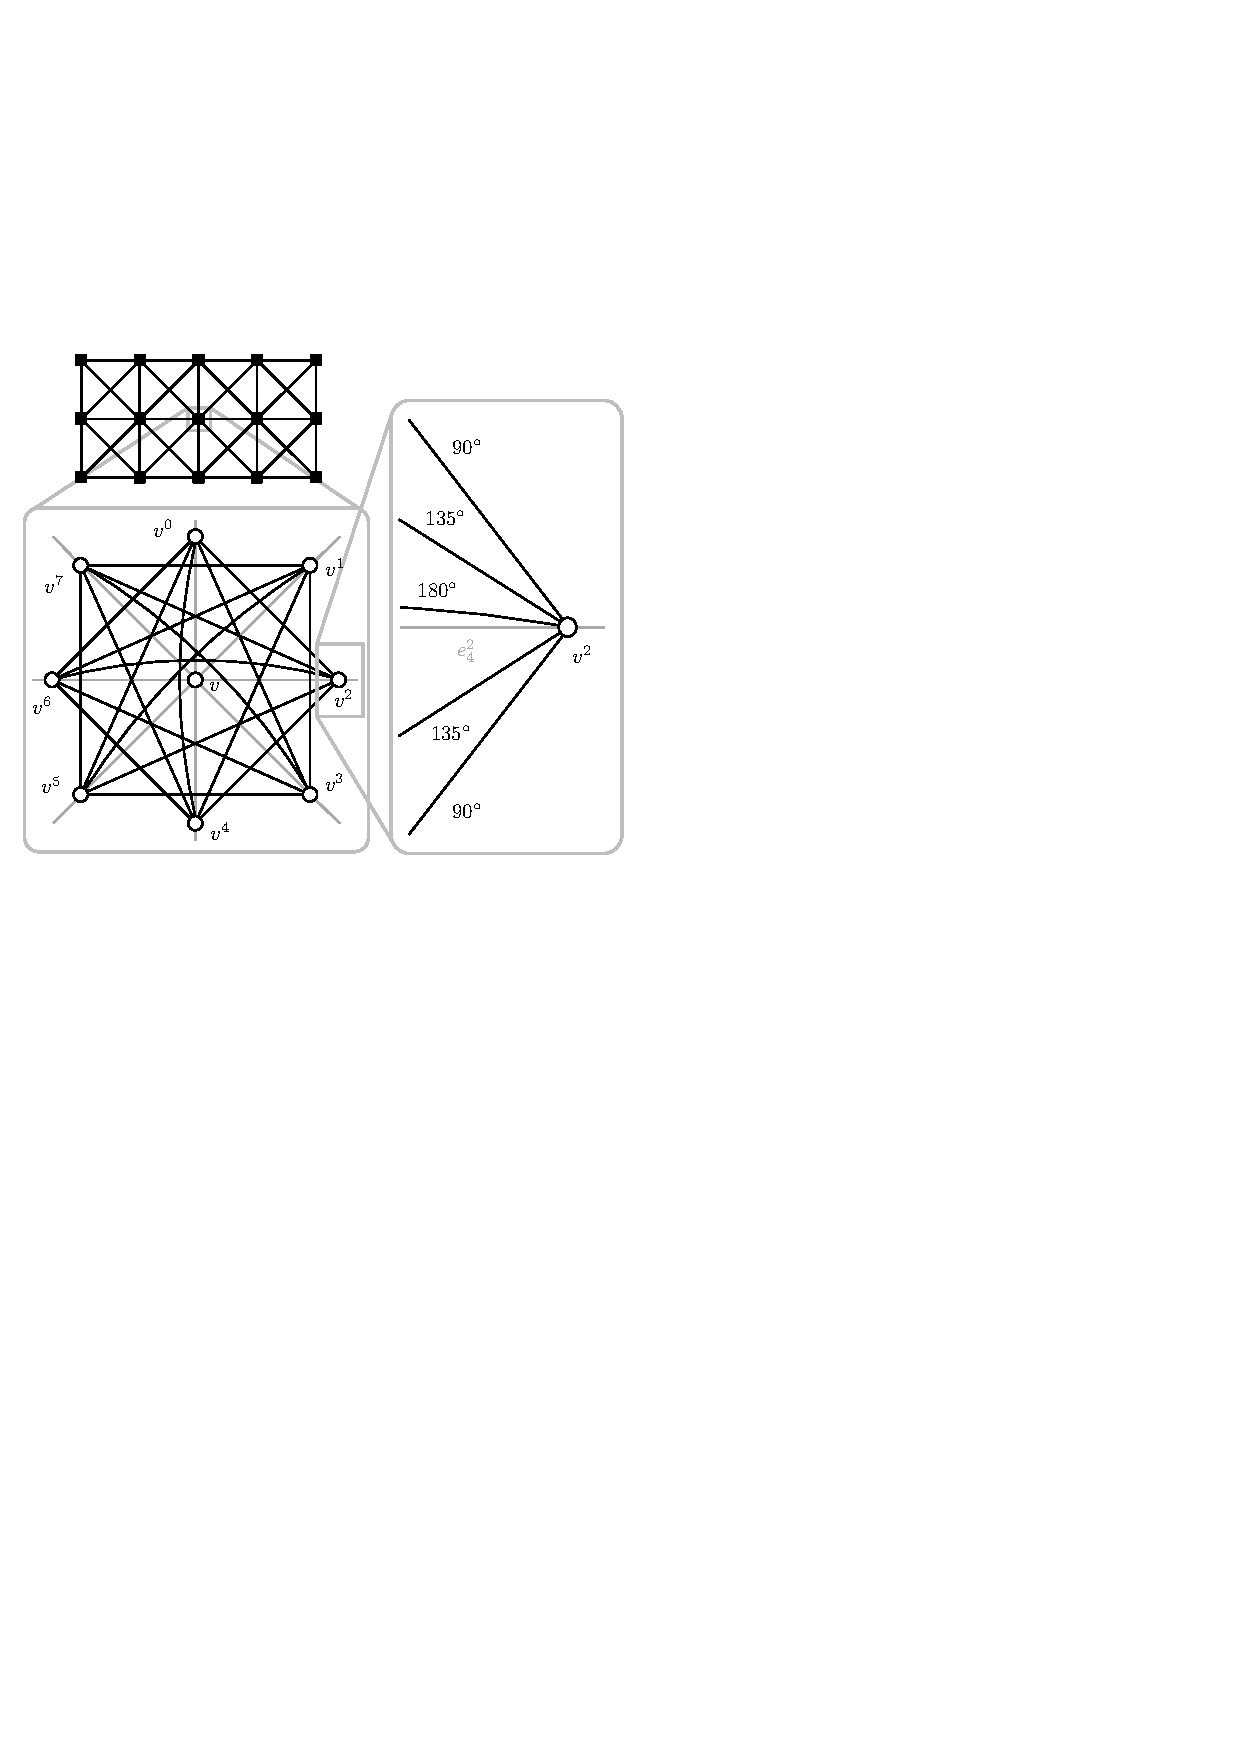
\includegraphics[width=0.45\textwidth]{figures/node.pdf}}}$
	\caption{A $3\times5$ octilinear grid graph. Each node $\psi_i$ has 8 ports $\psi_i^0 ... \psi_i^7$ which are connected to $\psi_i$ by a direct edge. Each port is additionally connected to its $180^{\circ}$, $135^{\circ}$ and $35^{\circ}$ neighbor ports.}
	\label{FIG:gridgraph}
\end{figure}

To be able to distinguish the different node and edge types, we define the set of original grid nodes as $\Psi^g \ni \psi_{x, y}$, the set of port nodes as $\Psi^p \ni \psi_{x,y}^i$, the set of turn edges as $\Omega^t \ni \omega_{x, y}^{i@\theta}$, the set of sink edges as $\Omega^s \ni \omega_{x,y}^i$ and the set of original grid edges as $\Omega^g$.
Note that $\Psi = \Psi^g \cup \Psi^p$ and $\Omega = \Omega^t \cup \Omega^s \cup \Omega^g$.

Additionally, for each $\psi \in \Psi$, we define $\psi^* \in \Psi^g$ as the original grid node belonging to $\psi$ (this may be $\psi$ itself).

As we want to prevent the use of sink edges in pass-through nodes, we set a uniform sink edge cost $c_s$ high enough so that a sink edge is always more expensive than a turn edge. 
In a shortest path from $s$ to $t$, the only sink edges are then a leaving sink edge adjacent to $s$ and an arriving sink edge adjacent to $t$.

\subsection{Modelling Edge Costs}

As both a $45^{\circ}$ port edge and a $90^{\circ}$ port edge may be substituted by cheaper edges, special care has to be applied to the modelling of the actual edge costs.
For example, a $45^{\circ}$ turn can be simulated by first passing $v_{x, y}$ on a $180^{\circ}$ port edge, and then again on a $135^{\circ}$ port edge (Fig.~\ref{FIG:paths}, 3).
As $p_{180} < p_{135} < p_{45}$, this path may be cheaper than $p_{45}$, undermining our penalty system. 
Similarily, a $90^{\circ}$ degree turn can be simulated by two cheaper $135^{\circ}$ port edges (Fig.~\ref{FIG:paths}, 4).

To prevent the shortcuts described above, we first introduce a constant $a \geq 0$ and set new port edge costs $c'_{180}, ..., c'_{45}$ as follows:
%
\begin{align}
	c'_{180} &= a + c_{180} = a \\
	c'_{135} &= a + c_{135} \\
	c'_{90} &= a + c_{90} \\
	c'_{45} &= a + c_{45}.
\end{align}
%
We choose $a$ in a way such that the following inequalities are fullfilled:
%
\begin{align}
	2a + 2c_{135} &\geq a + c_{90} \label{CONSTRS:sim90}\\
	2a + c_{135} + c_{90} &\geq a + c{45}\label{CONSTRS:sim45}.
\end{align}
Ineq.~(\ref{CONSTRS:sim90}) ensures that simulating a $90^{\circ}$ pass with two $135^{\circ}$ passes is never cheaper than $c_{90}$.
Ineq.~(\ref{CONSTRS:sim45}) ensures that simulating a $45^{\circ}$ pass with a $135^{\circ}$ pass and a $180^{\circ}$ pass is never cheaper than $c_{45}$.

The inequalities are fullfilled for $a = c_{45} - c_{135}$.

The shortest path $p'$ from an original grid node $s = \psi_0$ to another original grid node $t=\psi_n$ on our octilinear grid graph now consists of \emph{two} nodes for each original grid node: for the start and end node, the original node and a single port node appear in the path.
For pass-through nodes, a port node for arriving at and a port node for leaving the original grid node appears (w.l.o.g., we ignore the case where a turn edge is replaced by two turn costs with similar cost, as this does neither affect the final path on the grid graph, nor the cost of that path).

This shortest path $p' = (\psi_0, \psi_1, ..., \psi_n')$ thus always describes a path $p = (\psi^*_0, \psi^*_2, \psi^*_4, ..., \psi^*_{n})$ on the original grid graph with $|p| = n = |p'| / 2 = n' / 2$ and has the cost
%
\begin{align}
	c'(p') = 2 c_s + \left(n - 1\right) \cdot c_h + \sum_{i=1}^{n - 1} a + t\left(\psi^*_{2i - 2}, \psi^*_{2i+2}\right)\label{EQ:cost}.
\end{align}
%
To get rid of the constant offset $a$, we set $c_{135} = 1$, $c_{90} = 1.5$ and $c_{45} = 2$, which means $a = 1$.
If we then set the cost of a single grid edge $c_h = 1 = a$ and set the actual grid edge costs to $c'_h = c_h - a = 0$, we can rewrite Eq.~\ref{EQ:cost} as  
%
\begin{align}
	c'(p') &= 2 c_s +  \left(n - 1\right) \cdot c'_h + \sum_{i=1}^{n - 1} c_h + t\left(\psi^*_{2i - 2}, \psi^*_{2i+2}\right) \\
	     &= 2 c_s + \left(n - 2\right) \cdot c_h + \sum_{i=1}^{n - 1} t \left(\psi^*_{2i - 2}, \psi^*_{2i+2}\right) \\
	     &= 2 c_s + c(p) - c_h = c(p) + 2 c_s - 1.
\end{align}
%
As $p'$ minimizes $c(p) + 2 c_s - 1$, it also minimizes $c(p)$.

\begin{figure*}[h]
  \centering
	$\vcenter{\hbox{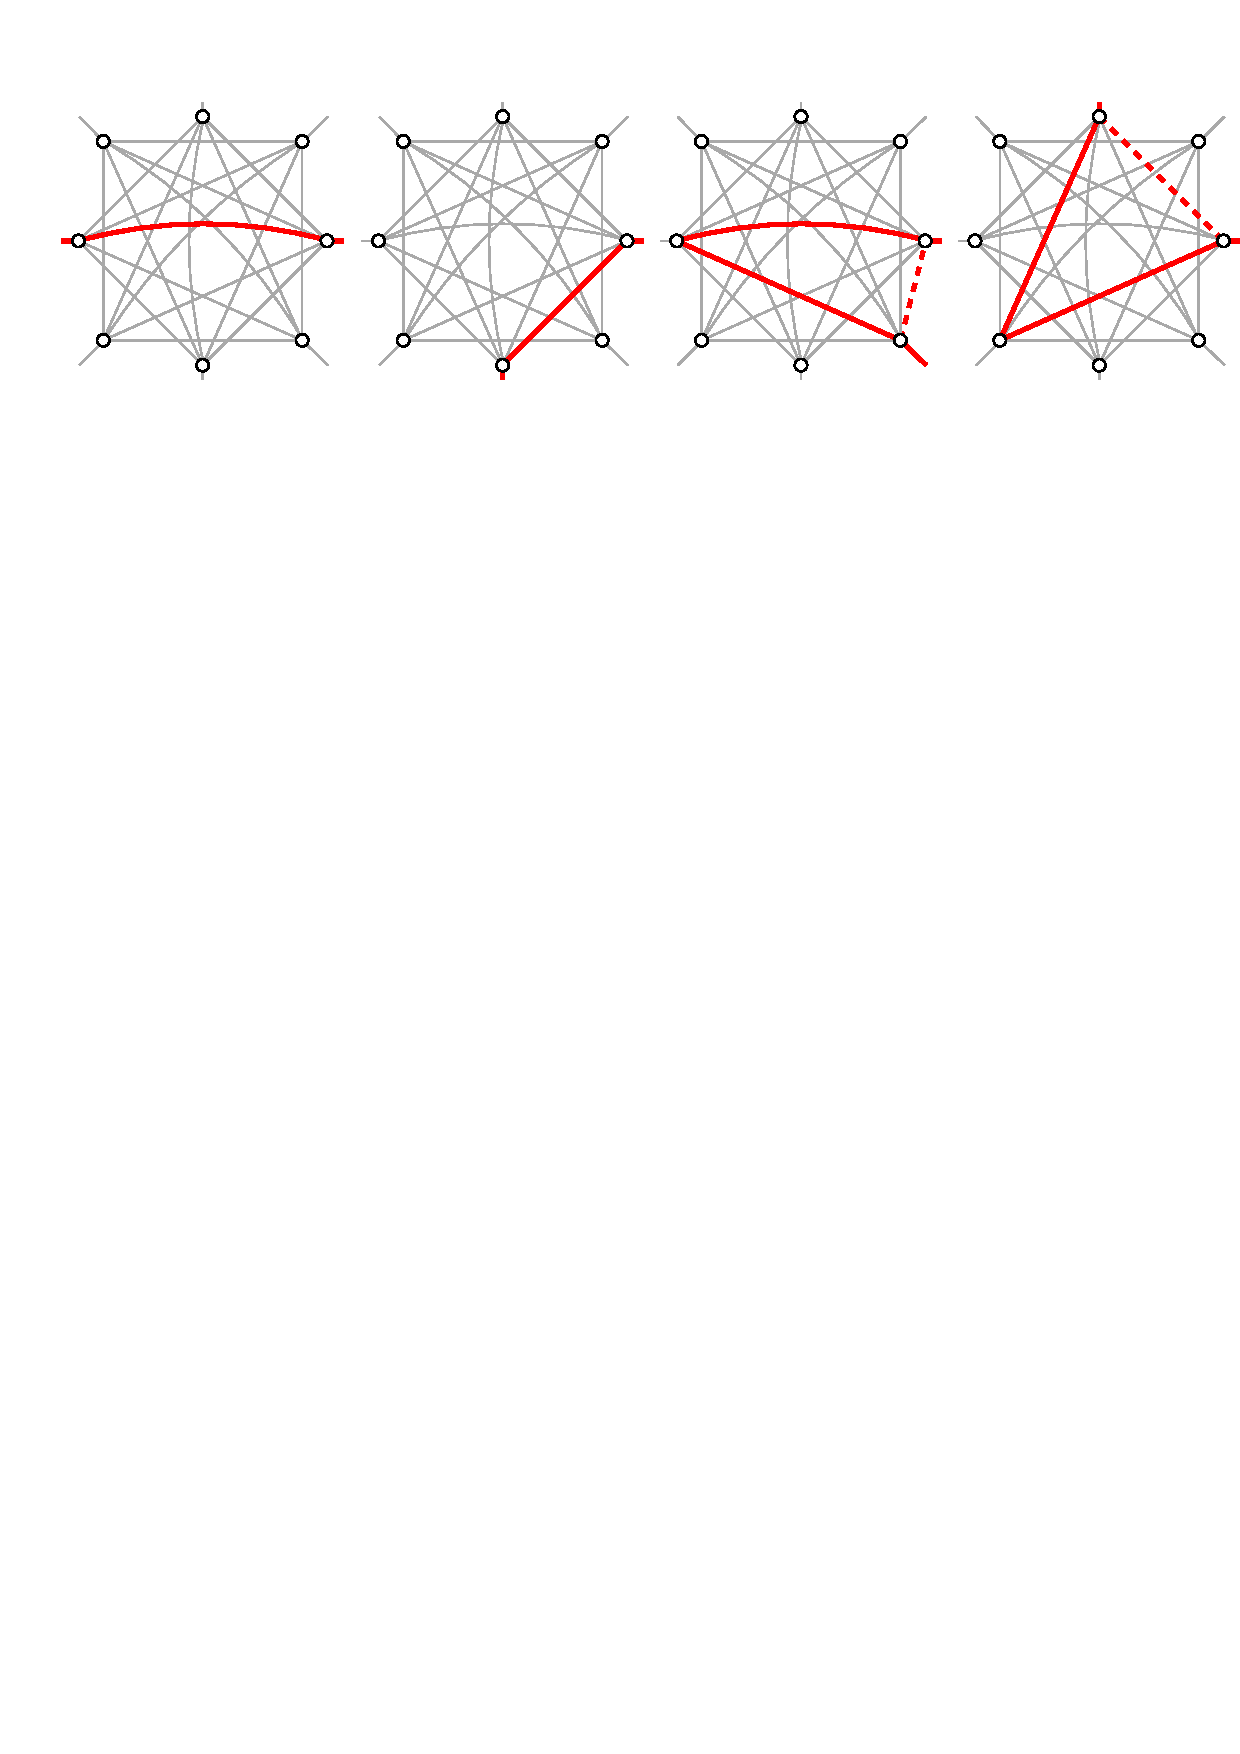
\includegraphics[width=0.9\textwidth]{figures/paths.pdf}}}$
	\caption{1. A $180^{\circ}$ pass through a node $\psi$. 2. A $90^{\circ}$ pass through $\psi$. 3. A $45^{\circ}$ pass through $\psi$ simulated by a $180^{\circ}$ and $135^{\circ}$ pass. 4. A $90^{\circ}$ pass through $\psi$ simulated by two $135^{\circ}$ passes. }
	\label{FIG:paths}
\end{figure*}

\section{Optimal Solution via ILP}

Using the octilinear grid graph $\Omega$ from the previous section, we can now define the problem of finding the optimal metro-map drawing on the grid defined by $\Omega$ like this: find the grid position for each input station and the shortest paths in the grid graph between adjacent input station nodes which minimizes the sum of (1) all shortest path costs, (2) the distance between the grid position of a station and its original position, and (3) the line bend penalties at stations (which are not covered by the path costs on $\Omega$).
The input embedding should be preserved, which means that the circular ordering of the input edges at nodes should be preserved, and the shortest paths should be non intersecting.

We first describe how to solve this problem exactly using an Integer Linear Program (ILP).

To make it easier to encode the direction of a shortest path from $s$ to $t$ in the ILP, we first model each undirected grid edge ${\psi, \psi'}$ as a pair of directed edges $(\psi, \psi')$, $(\psi', \psi)$.
This transforms our undirected grid graph into an equivalent directed grid graph.
Additionally, to get unique start and end nodes for the shortest path calculations, we now treat each undirected input edge $e = \{u, v\}$ as a directed edge $(s, t)$.
As the shortest paths in our octilinear grid graph are symmetric, it does not matter whether we chose $s = u, t = v$ or vice versa.

To be later able to deduce the placement of stations computed by our ILP, we introduce binary decision variables $x_{v\psi}$ for each input node $v$ and grid node $\psi$ which should be 1 of $v$ was assigned to $\psi$, or 0 otherwise.
To be able to deduce the course of the shortest path, we define binary variables $x_{e\omega}$ for each input edge $e$ and each grid edge $\omega$ which should be 1 if $\omega$ is used in the octilinear curve for $e$, or 0 otherwise.

We add $x_{e\omega}$ to the objective function with the cost of grid edge $\omega$ as a coefficient.

\subsection{Station Placement}

We have to ensure that each input station node $v \in V$ is assigned to exactly one grid node $\psi_{x, y} \in \Psi^g$, and that no two station nodes are assigned to the same grid node.
To achieve this, we first ensure that an input node is assigned to exactly one grid node with the following constraint:
%
\begin{equation}
  \forall v \in V: \sum_{\psi \in \Psi^g} x_{v\psi} = 1. \label{EQ:todo}
\end{equation}
%
An original grid node can either be assigned to a single input station, be used as a pass-through node for a single input edge, or be not used at all.
We encode this requirement with the following constraint:
%
\begin{equation}
  \forall \psi \in \Psi^g: \sum_{v \in V} x_{v\psi} + \sum_{e \in E} \sum_{\omega \in \Omega^p_\psi} x_{e\omega} \geq 1, \label{EQ:singleuse}
\end{equation}
%
where $\Omega^p_\psi$ is the set of port edges belonging to $\psi$. 
If $\psi$ is assigned to an input station, the first sum is already 1, forbidding the use of $\psi$ as a pass-through node for the curve of any input edge.
Similarily, if $\psi$ is used as a pass-through node, it cannot be assigned to an input station node.
As Equation~\ref{EQ:singleuse} cannot exceed 1, a grid node can then indeed only be assigned a single input node, be used by a single path as a pass-through node, or be not used at all.
Note that Equation~\label{EQ:singleuse} also enforces that a grid edge $\omega \in \Omega^g$ can only be used by a single path for an input edge, as a second path using $\omega$ would have to either arrive or cross a grid node that is already used by the other path occupying $\omega$, which Equation~\label{EQ:singleuse} explicitely prevents.

\subsection{Edge Continuity}

To globally compute the shortest paths on the grid graph between all adjacent input nodes, we make use of the standard formulation of the shortest path problem as a Linear Program.
We have to make sure that edges assigned to the shortest path from $s$ to $t$ are connected.
To ensure this, we introduce the following constraints per grid node and input edge:

\newcommand\Psum[1]{\sum_{\makebox[0pt]{$\scriptstyle#1$}}}

\begin{equation}
  \forall e \in E\ \forall \psi \in \Psi^p: \Psum{\omega \in \text{out}(\psi)} x_{e\omega} - \Psum{\omega \in \text{in}(\psi)} x_{e\omega} = 0. \label{EQ:cont_port}
\end{equation}
\begin{equation}
	\begin{split}
  	\forall e \in E\ \forall \psi \in \Psi^g: x_{t\psi} - 2x_{s\psi} + \Psum{\omega \in \text{out}(\psi)} 2x_{e\omega} - \Psum{\omega \in \text{in}(\psi)} x_{e\omega} = 0. \label{EQ:cont_grid}
  \end{split}
\end{equation}

Equation~\ref{EQ:cont_port} makes sure that the number of outgoing and incoming edges at each port node is the same.
This ensures a continuous path between the grid node chosen for $s$, and the grid node chosen for $t$.

Equation~\ref{EQ:cont_grid} handles the original grid nodes chosen for $s$ and $t$.
At these nodes, we count an outgoing edge twice, which means that the grid node could only make up for an outgoing edge with two incoming edges.
This, however, would mean that our shortest path split somewhere, which is prevented by Equation~\ref{EQ:cont_port}.
The only way to fullfill the constraint is thus for $\psi$ to be the source node for the input edge.
Similarily, the only way to counter an incoming edge is for $\psi$ to be the target node for the input edge.

\subsection{Preservation of Embedding}

To preserve the input embedding, it is enough to guarantee that no two paths in $\Gamma$ intersect and that the circular ordering of adjacent edges is the same as in the input graph.
Equation~\ref{EQ:singleuse} already prevents paths crossing at grid nodes.
There is now exactly one remaining case where paths in $\Gamma$ could create intersections: if two intersecting diagonal grid edges are used.
To prevent this case, we define $\Omega^d$ as the set of diagonal grid edges in $\Gamma$ and say that for $\omega \in \Omega^d$, $\omega^{\times} \in \Omega_d$ is the diagonal edge crossing $\omega$. 
We then add the following constraint:
%
\begin{equation}
  \forall \omega \in \Omega^d: \Psum{e \in E} x_{e\omega} + x_{e\omega^{\times}} \leq 1. \label{EQ:crossing}
\end{equation}

To ensure that the circular edge ordering at nodes remains the same, we would first like to have a variable $x_{ue} \in \{1, ..., 8\}$ which tells us the direction of input edge $e$ at adjacent input node $u$ in the final grid graph drawing.
To get the desired assignments, we add the following constraints:
%
\begin{equation}
  \forall e = (s, t) \in E: \sum_{\psi_{x, y} \in \Psi^g} \sum_{p = 1}^8 p x_{e(\psi_{x, y},  \psi_{x, y}^{(p - 1)})} - x_{se} = 0\label{EQ:dirfrom}
\end{equation}
\begin{equation}
  \forall e = (s, t) \in E: \sum_{\psi_{x, y} \in \Psi^g} \sum_{p = 1}^8 p x_{e(\psi_{x, y}^{(p - 1)}, \psi_{x, y})} - x_{te} = 0\label{EQ:dirto}
\end{equation}
%
In Equation~\ref{EQ:dirfrom}, each outgoing sink edge $(\psi_{x, y},  \psi_{x, y}^{(p - 1)}), p \in {1, ..., 8}$ adds $p$ to the sum.
As Equations~\ref{EQ:cont_grid} and \ref{EQ:singleuse} ensures that only a single outgoing sink edge in the grid graph may be used by the path for an input edge, we can be sure that the left side of the equation always exactly equals the octilinear direction $1, ..., 8$ of $e = (s, t)$ at $s$.
The only way to fullfil the constraint is thus to set the value of $x_{se}$ to the octilinear direction.
Equation~\ref{EQ:dirfrom} is modelled equivalently for paths incoming at $t$.

To finally ensure that the edge ordering in the final drawing matches the input drawing, we apply a trick originally used in \cite{noellenburg}.
If $\text{dir}(u, v)$ is the angular direction of $(u, v)$ in the drawing of input graph and if $v_1, ..., v_p, ..., v_{\text{deg}(u)}$ is the clockwise ordering of nodes adjacent to u in the original embedding, then $\text{dir}(u, v_p) < \text{dir}(u, v_{p + 1})$ has to be true for all but one $p \in \{1, ..., \text{deg}(u)\}$ in the final octilinear drawing.

This can be enforced with the following constraints:
%
\begin{equation}
  \forall u \in V, \deg(u) > 2: x_{v(v, u_{p + 1})} - x_{v(v, u_{p})} + 8\beta_p(v) \geq 1\label{EQ:dirs}
\end{equation}
\begin{equation} 
  \forall u \in V, \deg(u) > 2: \sum_{p = 1}^{\deg(u)} \beta_p(v) \geq 1\label{EQ:onedev}.
\end{equation}
%
If $\text{dir}(u, v_p) \not< \text{dir}(u, v_{p + 1})$, then $x_{v(v, u_{p + 1})} - x_{v(v, u_{p})} \leq 0$ and the only way to fullfill Equation~\ref{EQ:dirs} is to set $\beta_p(v)$ to 1.
Equation~\ref{EQ:onedev} ensures that this can only happen a single time.

\subsection{Avoiding Line Bends}

As our shortest path calculations only penalize line bends along paths, we additionally have to ensure that line bends at input nodes are equivalently penalized.
We would like to have variables telling us wither edges $e$ and $f$ in the original input graph describe a $45^{\circ}$, $90^{\circ}$, $135^{\circ}$ or $180^{\circ}$ at their joint node (as $G$ is not a multigraph, this joint node is unique).

We first note that for two directional variables $x_{ue}$ and $x_{uf}$, $x_{ue} - x_{uf} \mod 8$ is either 1 or 7 for $45^\circ$ bends, 2 or 6 for $90^\circ$ bends, 3 or 5 for $135^\circ$ bends and 4 for $180^\circ$ bends.

As modulo cannot be used directly in an ILP, we use the following constraint for each pair $e, f$ of edges in the input graph adjacent at node $u$ and sharing a common line:
\begin{equation} 
  0 \leq x_{ue} - x_{uf} + 8 \gamma_{ef} \leq 7.
\end{equation}

The auxiliary variable $\gamma_{ef}$ will be 1 if $x_{uf} > x_{ue}$. As both $x_{ue}$ and $x_{uf}$ are in the range $[1, 8]$ and as $x_{ue} \neq x_{uf}$ (per Eq.~\ref{EQ:singleuse}), we then have $x_{def} = x_{ue} - x_{uf} + 8 \gamma_{ef} = x_{ue} - x_{uf} \mod 8$.

We then add the following constraint for each of the input edge pairs:
%
\begin{equation} 
  x_{def} - x_{ef}^{45} - 2x_{ef}^{90} - 3x_{ef}^{135} - 4x_{ef}^{180} - 5 {x'}_{ef}^{135} - 6{x'}_{ef}^{90} - 7{x'}_{ef}^{45} = 0.
\end{equation}
%
To make sure that only one of the bend variables is set to 1, we add the following constraint:
%
\begin{equation} 
  x_{ef}^{45} + x_{ef}^{90} + x_{ef}^{135} + x_{ef}^{180} + {x'}_{ef}^{135} + {x'}_{ef}^{90} + {x'}_{ef}^{45} = 1.
\end{equation}
%
Each of the 8 bend variables is then added to the objective function with its corresponding penalty.

\subsection{ILP Complexity}



\section{Approximative Solution}

\subsection{Station Placement}

\subsection{Edge Continuity}

\subsection{Preservement of Embedding}

\subsection{Avoiding Line Bends}

\subsection{Optimization via Local Search}

\subsection{Complexity}

\section{Evaluation}

\subsection{Penalty Experiments}

\section{Conclusions}


\balancecolumns
\end{document}
